\chapter{Research Papers}
\label{chap:research-papers}

\underline{\textbf{Objective question for Research:-}}

% This explanation is for the PSSW related papers.
% \large{Does a static magnetic field contribute to the excitation of perpendicular standing spin-wave (PSSW) modes, and can this contribution be identified from the results of this work?}

% This explanation is related to the Exchange bias based papers.
Look for exchange bias in the $\mathrm{CoFe/FeO}$ bilayer, then try changing the interface damping and the anisotropy value, and varying the thicknesses of the ferromagnetic (FM) and antiferromagnetic (AFM) layers.


\section{FMR studies of surface and bulk spin-wave modes in a CoFe/PtMn/CoFe multilayer film - \href{http://dx.doi.org/10.1063/1.2839337}{JAP 103, 07B525 (2008)}}
\subsection*{Main points from the Paper}
\begin{enumerate}
    \item Studied the exchange-dominated surface and bulk spin-wave modes in a single period of CoFe/PtMn/CoFe trilayer film.
    \item Multimode spin-wave spectra was observed using the FMR. Also, they have identified a high-order standing spin wave in the spectra and found \textbf{"critical angle"} in the multilayer sample. They have also included the effective surface anisotropy field to describe the results.
    \item They have used FMR to investigate the exchange-dominated surface and bulk spin-wave modes in a single period of CoFe/PtMn/CoFe tri-layer film. Bulk magnetic anisotropy parameters and the g-factor of the magnetic film based on the angle dependence of the main resonance field.
    \item A significant enhancement in the in-plane anisotropy was observed in the range; $\sim57-123$ Oe.
    \item A high-order standin spin wave was identified in our spectra along with a "critical angle" in the trilayer sample. 
    \item An effective surface anisotropy field due to the exchange bias and the dynamic surface spin pinning was also used to describe the results.
    \item The exchange interaction stiffness in the CoFe layers, $J\sim 2.7$ meV.
    \item \underline{Acoustic spin-wave mode:} The acoustic spin wave mode is the lowest-frequency mode where all spins in the material move together and stay in phase across the thickness. e.g. In a thin ferromagnetic film, all magnetic moments tilt and precess together when a microwave field is applied.
    \item \underline{Higher-order standing SW:} Higher-order standing spin wave modes occur when spins form standing patterns across the thickness, with some regions moving opposite to others. e.g. In a thick magnetic film, the magnetization oscillates with one or more nodes across the thickness, similar to standing waves on a stretched string.
    \item These results could be related to the change of surface spin pinning is also said in the paper.
    \item A two-fold symmetry for the out-of-plane geometry is observed when the angular dependence of the resonance filed of the acoustic spin-wave mode is measured.
    \item The excitation of the spin-wave precession is due to the absorption of microwave. 
    \item The effective parameter A changes with changing angles when we rotate the sample, and the magnetic profile changes due to the change of the surface pinning. This results in the change of the spin-wave resonance energy.    
\end{enumerate}
\subsection*{Summary}
In summary, we investigated the basic magnetic excitations in a CoFe/PtMn/CoFe multilayer film using the FMR technique. A higher-order spin-wave mode appears only after the magnetic field is tilted beyond a certain angle. By considering an effective surface anisotropy field, the observed spin-wave resonance spectra can be explained by dynamic pinning of spins at the surfaces.


 %2008 PSSW paper
\section{Perpendicular standing spin wave and magnetic anisotropic study on amorphous FeTaC films - \href{https://doi.org/10.1109/TMAG.2016.2520981}{TMAG 7 52, 2520981 (2016)}}

\begin{description}
    \item[\underline{Perpendicular Standing spin-wave (PSSW):}]A perpendicular standing spin-wave is a magnetic excitation in a thin film where the spins oscillate in a standing-wave pattern across the film thickness, that is, perpendicular to the film surface.

    E.g: In a thick ferromagnetic film measured by FMR, higher-order resonance peaks appear because the magnetization forms standing waves between the two film surfaces.
\end{description}
\subsection*{Main points from the Paper}
\begin{enumerate}
    \item Magnetic anisotropy, spin wave (SW) excitation, and exchange stiffness constant of amorphous $\mathrm{Fe_{80}Ta_8C_{12}}$ $(d=20 - 200 \mathrm{nm})$ films were studied as a function of thickness using microstrip-FMR.
    \item The amorphous nature of the soft ferromagnetic (FM) alloys has no grain boundaries, which is important for the magnetization reversal and enhances the speed of spin-switching in spin transfer torque devices.
    \item In the case of FMR, the external microwave field couples with uniform and nonuniform SW modes. This excitation of magnetistatic modes occurs especially in dipole-dipole interaction dominated system where the wave vector $(\vec{q})$ lies in the plane.
    \item The modes with wave vector $(\vec{q})$ component perpendicular to the film surface is termed perpendicular standing spin-wave (PSSW) modes and the quantization of these modes is due to the geometrical confinement \cite{gui2007quantized}. 
    \item According to the Kittel model, the excitation of odd SW modes can be observed with the spin pinned by surface anisotropy interaction. However, in the case of partially surface pinned spins, both even and odd SW modes can be excited.
    \item The magnetic field sweep FMR spectra were carried out for different precessional frequencies and azimuthal angles.
    \item By increasing the thickness of the film $(\geq100 \mathrm{nm})$, $M-H$ curve clearly shows the transcritical loop manifesting the presence of stress-induced perpendicular anisotropy during the film deposition.
    \item The room temperature soft magnetic properties degrade drastically as the thickness increases due to the transition from the in-plane orientation of magnetization to the strip domain patterns.
    \item At the thickness of 20 nm a clear uniform precession mode without any other SWR mode in which the dynamic magnetization is uniform across thickness. 
    \item However, when the thickness is increased from 50 nm onward, the first PSSW mode is excited at lower absorption fields. The signal strength is 7 times smaller than the uniform mode.
    \item The absence of the higher order $(n>1)$ exchange-dominated PSSW modes could be due to very weak excitation, and the intensity of those nodes may be lower than our detection sensitivity.
    \item The increasing differences between the first PSSW modes and the uniform mode, could be understood on the basis of perpendicularly quantized SW vector, which is inversely proportional to the film thickness, i.e., $q=n\pi/d$.
    \item The angular dependence of resonance fields is governed by uniaxial magnetic anisotropy, in the case of 20 nm, $\phi_H$ dependence of $H_r$ for uniform mode at 6, 8 , and 10 GHz precessional frequencies.
    \item The typical field dependence of the resonant frequencies are shown in fig: 3(b). \hl{Watch this in detail}.
    \item The origin of in-plane uniaxial magnetic anisotropy in FeTaC thin films $(d=20$ and $50$ nm$)$ could be understood on the basis that the strong exchange coupling between the FM atoms plays an important role during the deposition process, which allows to form aligned FM atom pairs parallel to the film plane. 
    \item On further increase of the thickness, the in-plane uniaxial magnetic anisotropy disappears. 
\end{enumerate}
\subsection*{Summary}
The MS-FMR method was used to study magnetic anisotropy and spin-wave excitations in soft ferromagnetic FeTaC films. The angular variation of the resonance field within the film plane indicates a weak uniaxial anisotropy for films with thicknesses of 20 and 50 nm. Along with the uniform precession mode, the observation of the first perpendicular standing spin-wave mode confirms the role of both exchange and dipolar interactions. The exchange stiffness constant of these amorphous films was obtained from the in-plane angular behavior and from the frequency separation of the PSSW mode measured along the easy and hard magnetization directions. The extracted exchange stiffness increases from $2(4)\times10^{-7} \mathrm{to} 3.5(5)\times10^{-7}$ erg/cm as the film thickness increases from 50 to 200 nm. % 2016 ANjan Barman PSSW paper
\section{Perpendicular standing spin waves in AuPt/GdFeCo induced by spin-orbit torques - \href{https://doi.org/10.1038/s42005-025-02433-2}{Comm. Phys.,8, 516 (2025)-Nature}}

\section*{Main points from the Paper}
\subsection*{\underline{I. Introduction:}}
    \begin{enumerate}[1.]
        \item GdFeCo has a ferrimagnetic compositions, their spin dynamics in the present regime are effectively ferromagnetic (FM).
        \item They have observed the SOT, generated from the adjacent AuPt layer induce perpendicular standing spin waves in GdFeCo, with resonant modes observed up to the third order. 
        \item Uncapped films exhibit oxidation-induced degradation that suppresses spin-wave confinement and to avoid that they have used Ta as the capping layer. 
        \item Ferrimagnetic materials (FiMs) can also be used to provide most of the things which are useful in device chips which require a faster switching speeds and reduced saturation magnetization [\textcolor{red}{first lines are good}].
        \item The combined properties of FM and AFM are found in the FiMs: low net saturation magnetization, fast magnetic dynamics driven by antiferromagnetic precession, and the ease of magnetization manipulation and detection typically seen in ferromagnets.
        \item Because of the presence of the forced precession of antiparallel spins in FiMs, there is formation of perpendicular standing spin-waves(PSSW) modes, where spins oscillate perpendicular to the film surface.
        \item The formation of PSSW modes was observed recently in AFM or FiM systems in connection with FM which is attributed to the interlayer exchange coupling with the adjacent FM layer. 
        \item ST-FMR is used to observe the PSSW modes in AuPt/GdFeCo.
        \item In the case of uniform precession of the magnetic moments $(p=0)$ or PSSW modes when spin waves witht non-zero wave vectors satisfy the confinement condition \boxed{$(k=p\pi/d)$} where $d$ is the film thickness.
        \item The Ta capping layer was used as capping layer to reduce the oxidation and enabled us to stabilize the PSSW modes up to the $p=3$. And the samples without the Ta capping, the ST-FMR spectra with PSSW modes were limited to the $p=2$ and a reduced saturation magnetization compared to those with the Ta capping layer.
        \item These findings provide valuable insights for the development of FiM-based SOT-MRAM and logic devices, which benefit from the unique properties of FiMs.
    \end{enumerate}
\subsection*{\underline{II. Results and Discussion:}}
\begin{enumerate}[1.]
    \item VSM is used to measure the fundamental magnetic properties of the system, and saturation magnetization $(M_s)$ and effective anisotropy energy density $(K_{eff})$ as a function of GdFeCo thickness is calculated. \footnote{See the supplementary note 1 of the paper for detailed calculations of these.}
    \item Surface effects was taken as the reason why there is larger saturation magnetization $(M_s)$. On increasing thickness, the bulk properties becomes more dominant enhancing ferrimagnetic ordering and a reduction of overall magnetization.
    \item Suppression of oxidation significantly affects the magnetization, particularly at lower thicknesses.[\textcolor{red}{Important Line}]
    \item Surface anisotropy weakens as $t_{GdFeCo}$ increases, leading to bulk anisotropy becoming dominant contribution. It is consisted with $M_s$ results.
    \item No PMA has been observed across the entire thickness range.
    \item The spin currents generated by the Spin Hall Effect (SHE) from the strong SOC in the adjacent AuPt layer and the induced $H_{Oe}$ produced by the RF current drives the magnetization dynamics in the GdFeCo layer, where the antiparallel alignment of magnetic moments results in varying precession amplitudes and directions among individual atoms.
    \item The excited spin-wave modes generated by this dynamic behavior exhibit the PSSW modes when teh wave vectors $(k)$ satisfy the confinement condition, $k=p\pi/t_{GdFeco}$.
    \item The Ta layer prevents the formation of FeO, CoO, or GdO hence the 3rd mode $(p=3)$ is only present in the case of Ta capping.
    \item Experimental evidence of presence of 3rd PSSW mode in the presence of the Ta layer was observed. This enhances the surface pinning and spin-wave reflection, promoting the formation of higher-order PSSW modes.
    \item The sharp increase in $(A_{ex})$ at $t_{GdFeCo}=80$ nm is attributed to the dominant bulk properties in the GdFeCo layer. This irregular behavior suggests that spin-wave propagation and PSSW formation are hindered by spin-wave absorption and reduced spin-wave reflection due to surface oxidation.
    \item The interfacial engineering after adding Ta as the capping layer, stabilizes the ferrimagnetic dynamics, promoting the formation of higher-order spin-wave modes.
    \item The dynamic pinning model and introduced the wave vector$k_p$ defined as $k_p=\left[\frac{(p+\delta)\pi}{t_{GdFeCo}}=\frac{2\pi}{\lambda_p}\right]$, where $\lambda_p$ is the wavelength in the GdFeCo layer, accounting for each mode  $p$ and the pinning parameter $\delta$ was used by the authors to quantify the degree of pinning at the surface. [\textcolor{red}{ref. 49-51, from this paper}].
    \item When the Ta capping was done on the system here, this pinning model specified that there is strong interfacial confinement and in the case of not Ta capping, there was significantly lower confinement.
    \item Conclusively, the Ta capping enhances the interfacial confinement, supporting the formation of stable and higher-order PSSW modes.
    \item When magnetic field polarity measurements were carried out, the 1st PSSW mode was only visible under a positive external magnetic field. In contrast, the Ta-capped samples exhibit symmetrical resonance under both positive and negative external fields. 
    \item The oxidation of the Gd leads to the asymmetrically aligned local magnetic moments, breaking the mirror symmetry with respect to the external magnetic field.
    \item Potential mechanisms may include non-reciprocal spin-wave propagation in magnetization-graded systems or the influence of the Dzyaloshinskii-Moriya interaction (DMI) [\textcolor{red}{ref. 56-59 from this paper}]. 
\end{enumerate}
\subsection*{\underline{III. Summary:}}
\begin{enumerate}
    \item An investigation of the formation of PSSW modes in ferrimagnetic GdFeCo layers drive by SOTs generated by the adjacent high SOC material, AuPt was carried out.
    \item The ST-FMR spectra explains the induced antiparallel magnetization precession after the contact of AuPt which injected the SOT.
    \item Oxidation at the surface of GdFeCo was shown to significantly affect the key properties such as $M_s,A_{ex}$, and overall quality of deposited GdFeCo layer.
    \item The pinning effects at the interfaces were evaluated using a dynamic pinning model, demonstrating that the Ta-capped samples provided strong interfacial confinement for PSSW modes, while the uncapped samples exhibited relaxed boundary conditions and weaker pinning.
\end{enumerate}
 % 2025 Very recent PSSW paper AuPt/GdFeCos
\section{Perpendicular standing spin waves in films with interfacial Dzyaloshinskii-Moriya interaction - \href{https://doi.org/10.1103/PhysRevB.111.064432}{PRB, 111, 064432 (2025)}}

\section*{Main points from the Paper}
\subsection*{\underline{I. Introduction:}}
\begin{enumerate}
    \item As Dzyaloshinski Moriya interaction (DMI) is known to induce the nonreciprocity in spin wave propagation within the plane of magnetic thin films.
    \item Analytical expressions are developed to estimated the effecets of DMI on spin waves by assuming the magnetization dynamics are uniform throughout a film thickness.
    \item The calculations done here show that the PSSW mode frequencies depend nonlinearly on the interfacial DMI strength and on the inverse thicknesses of the magnetic films.
    \item DMI is an antisymmetric exchange interaction caused by spin-orbit coupling and broken symmetry that enforces a preferred rotational sense in magnetic textures and their stabilization. It exists when the following conditions are met:
    \begin{enumerate}[\ding{212}]
        \item Strong spin-orbit coupling (usually from heavy metal).
        \item Broken inversion symmetry (typically at an interface).
    \end{enumerate}
    \item Generally Spin waves are the fundamental excitations of magnetic materials. 
    \item Spin waves in thin films are affected by interfacial DMI, leading to exciting phenomena such as nonreciprocal propagation, spin wave focusing, and even the loss of standing wave modes[\textcolor{red}{ref. 17-19}].
    \item Spin waves do provide the tool to measure the DMI experimentally \cite{stashkevich2015experimental,nembach2015linear}.
    \item Usually, in the theoretical studies of spin waves affected by DMI have assumed that the magnetization is uniform through the magnetic film's thickness \cite{moon2013spin,cortes2013influence}.
    \item The atomic layer method has been used to treat antiferromagnetically coupled stacks of thin films, exchange spring bilayers, and thin films with magnetoelectric coupling at interfaces \cite{moore2014spin}.
\end{enumerate}
\subsection*{\underline{II. Results and Discussion:}}
\subsubsection*{\centering A. One FM material}
\begin{enumerate}
    \item In the case of single FM material, it is assumed that the magnetization precession is uniform through the film.
    \item The full dipolar contribution is also included in the dispersion relation in Ref. \cite{moon2013spin}.
    \item The interfacial atomic DMI constant $D_{at}=4.2$ mJ$/m^2$ acts at the top layer only, which corresponds to an effective DMI used in the analytic expression of $D_{\mathrm{eff}}=D_{\mathrm{at}}/N=1.05$ mJ$/m^2$.
    \item The presence of DMI results in a pinning of a PSSW modes at the top surface, which is undetectable. The pinning is different for spin waves depending on the sign of $k_x$.
    \item One can see that without DMI, the mode is truly uniform through the film thickness, but with DMI and depending on the sign of $k_x$, the pinning results in nonuniform precession.
    \item Higher order standing spin waves are extremely sensitive to DMI because their motion is strongly confined across the film thickness, causing DMI and exchange to interact in a complex, non-additive way.
    \item It is well studied that increasing the thickness $L$ of a film will decrease the exchange energy and will therefore decrease the frequencies of higher-ordered PSSW [\textcolor{red}{ref. 36 \& 37}].
    \item The interface modifies the mode which then modifies the exchange interactions. And as a result, the frequency and damping is also modified. In our case this explains the non-monotonic damping trends.
    \item \hl{The system transitions from uniform-mode dynamics to exchange-dominated multi mode dynamics with increasing thickness}.
\end{enumerate}
\subsubsection*{\centering B. Two FM material}
\begin{enumerate}
    \item Interface position matters more than the interface strength. MgO interface is on one side only which introduces the asymmetry. Boundary conditions produce mode reshaping similar to FM bilayers.
    \item MgO in the case of my system can modify the local exchange interactions, orbital hybridization, and magnetoelastic coupling. Hence, the system behaves like a soft-hard exchange bilayer, even if chemically single phase. This justifies clearly the thickness dependent PSSW appearance in my work. [\textcolor{red}{V. Imp Line}]
    \item Thin films \ding{213} interface dominates \ding{213} uniform mode only.
    \item Thick films \ding{213} exchange resolved \ding{213} asymmetric standing modes appear.
    \item Novelty can be claimed on following points;
    \begin{enumerate}[\ding{212}]
        \item Mode-dependent damping
        \item Thickness-dependent transition from uniform to exchange-dominated dynamics.
        \item Interface-controlled PSSW emergence without explicit DMI.
    \end{enumerate}
\end{enumerate}
\begin{physicsmodule}{Related to my Paper}{Brown}
  \begin{lawbox}
    \subsection*{\sffamily\bfseries CoFe/MgO}
    \ding{212} In thicker CoFe films, perpendicular standing spin-wave modes emerge due to enhanced exchange confinement across the film thickness. These higher-order modes exhibit strong sensitivity to interfacial effects arising from the CoFe/MgO interface. Although such interfacial contributions are localized, they modify the standing-wave profile, leading to a nonlinear coupling between exchange-dominated dynamics and interface-induced fields. As a result, higher-order PSSW frequencies and damping respond more strongly than the uniform mode, consistent with the emergence of mode-dependent dynamic behavior at larger thicknesses.

    \ding{212} For CoFe/MgO, MgO modifies the exchange near the interface, and local anisotropy. This directly affects PSSW formation and damping.

    \ding{212} Studies of multilayer ferromagnetic systems have shown that perpendicular standing spin-wave modes become strongly asymmetric when magnetic properties vary across the film thickness. In such cases, interfacial effects modify the standing-wave profile rather than contributing as simple additive fields, leading to a nonlinear coupling between exchange-dominated dynamics and interface-localized interactions. As a result, higher-order PSSW modes exhibit enhanced sensitivity to interfacial asymmetry, making them effective probes of exchange nonuniformity and boundary conditions. Similar considerations apply to single-layer systems with asymmetric interfaces, where the emergence of higher-order modes reflects a transition from uniform-mode to exchange-resolved dynamics with increasing thickness.
  \end{lawbox}
\end{physicsmodule}
% \subsection*{\underline{III. Conclusion:}} % 2025 Very recent PSSW paper related to DMI
\section{Standing spin waves in Permalloy-NiO bilayers as a probe of the interfacial exchange coupling \href{https://doi.org/10.1103/PhysRevApplied.21.064044}{[\textit{Phys. Rev. Appl., 21 064044 (2024)}]}}

\subsection*{\underline{Abstract}}
The importance of ferromagnetic-antiferromagnetic (FM-AFM) bilayer dynamics, with emphasis on the interaction occurring at the interface, where the magnetic moments of the AFM can be imprinted into the FM, and the exchange bias field can affect these dynamics, is explained in this paper. Here, in this paper, they have used Permalloy (Py) and NiO (Py/NiO) hybrids, and for comparison, single Py films in the broad Py thickness range varied from a few nm to 200 nm by using static (Kerr effect) and dynamic (spin-wave) measurements along with micromagnetic simulations. Uniform precession and perpendicular standing spin waves (PSSWs, $n=1, 2)$ and a clear enhancement of the PSSW mode frequencies upon interfacing Py with NiO, both from experiments and simulations.

\hspace{1cm}The enhancement of the mode frequencies with increasing the thickness of the material, which explains its interfacial origin rooted in the exchange coupling between the FM and AFM layers. \hl{Their results suggest that PSSW detection in a ferromagnet offers a means of probing the interfacial exchange coupling with the adjacent AFM layer}. Furthermore, the controlled spatial symmetry breaking by the AFM layer enables engineering of PSSWs with different spatial profiles in the FM.

\subsection*{\underline{Introduction}}
\begin{enumerate}
    \item The focus on the investigation of ferromagnet-antiferromagnet (FM-AFM) bilayers has been concerned with the induction of uniaxial anisotropy, and recently, a thin FM layer coupled with a thick AFM layer was also studied to observe the AFM spintronics. An important factor present in both of them is the exchange coupling at the AFM-FM interface, since it's not only the shifts that we get in the static hysteresis curves, but it may also affect magnetization dynamics.
    \item Excitation of spin waves (SWs) in a FM coupled to AFM was proposed method to propagate spin excitation into the AFM \cite{jenkinsSpinWaveExcitations2020}.
    \item Recently, PSSWs have been studied in other symmetry-breaking systems like heavy metals-magnetic insulator (HM-MI) bilayers, where the frequency of the standing-wave modes experiences a shift \cite{lee2023erratum}. The effect was attributed to an additional confinement of the waves upon a local increase of the interfacial damping due to spin pumping \cite{lee2023erratum}.
    \item There are other experiments also, as per this paper, which have used PSSWs to probe coupling in FM bilayer or individual surface anisotropies on epitaxial FM layers with nonequivalent interfaces [\textcolor{red}{ref. 10-13,14}]. 

\hl{The introduction part is written in a perfect way. Please read it and get the references. Try to get the exchange length of the CoFe (B2-CsCl structure).}


    \item Lower $M_s$ is set near the top surface of our films. This translates to a lower demagnetizing field and a higher effective potential in these layers, thus enabling the pinning of the PSSW mode. [\textcolor{red}{ref. 30}].
    \item This effect might also be due to the surface oxidation typically experienced by ferromagnetic films or a magnetization symmetry breaking in the normal direction due to a capping layer.
    \item In the case of Py, the variation in the $M_s$ is the most conceivable way to induce changes in the surface pinning parameter \cite{waring2023exchange}, therefore generating magnetization symmetry breaking and allowing the excitation of PSSWs.
    \item The averaged out-of-plane (OOP) magnetization of the system was converted into the frequency domain after the use of a Fourier transform \cite{park2003imaging}. This process was repeated for each of the presented magnetic fields.
\end{enumerate}

\subsection*{\underline{Experimental Results \& Discussion}}
\begin{enumerate}[A.]
    \item \underline{Static Characterization of the Py and Py/NiO films:}
    \begin{enumerate}[1.]
        \item Static MOKE reveals the clear enhancement of the ferromagnetic films upon the addition of NiO. As expected, there is an exchange bias in the FM/AFM layer.
        \item Experimentally, it has been proved that this phenomenon will suppress once the thickness of the FM layer becomes large enough, which can be attributed to the reduced effect of the interface exchange coupling strength relative to the overall magnetization of the film.
        \item They have also observed the shift in the hysteresis loops from a field-centered position, which clearly indicates the presence of an exchange bias field in Py/NiO.
        \item There is also a reduction in the exchange bias field as the Py layer becomes thicker, once again, an effect related to the reduced influence on the overall film magnetization. \hl{Quantifiable exchange coupling within our AFM-FM films}
    \end{enumerate}
    \item \underline{Effect of NiO on the frequency of the observed standing waves}
    \begin{enumerate}[1.]
        \item After doing the VNA-FMR, they have observed a uniform FMR mode, characteristic of the FM layers in the case of both Py and Py/NiO.
        \item The spin-wave modes are identified as exchange-dominated thickness-dependent modes related to PSSWs in our films \cite{dabrowski2021canted}.
        \item The existence of different PSSW modes with the thickness of the films is also observed. 
        \item In this system, the PSSW modes were shifted to higher frequencies, replacing the standing spin-wave modes. The frequency shift decreases with the enhancement of the thickness of the Py layer.
        \item This suggests that there is a direct relation between the magnitude of the magnetic moments in the film as the FM layer grows thicker and the frequency shift of the PSSW modes experienced when the NiO layer is added.
        \item Generally, FMR mode is independent of the thickness; however, in this case, when the thickness is increased, they have observed the frequency shift in the same direction for all of the pairs of samples.
        \item The frequency shift experienced by our films is a direct consequence of the Py magnetic moments pinning at the interface due to the exchange bias. The absence of free spins results in an additional confinement of the PSSWs.
        \item There is the confinement of the PSSW modes when the thickness is reduced to 2 nm, and it is supported by the experiments done on thin films.
        \item The saturation magnetization remained consistent at all thicknesses in the case of Py/NiO.
        \item The anisotropy field progresses similarly to the exchange bias and coercive fields extracted from the static hysteresis loops. This is expected since the exchange bias of the films has less influence on the overall magnetization as the film thickness increases.
        \item There is an increase of Gilbert damping (almost an order of magnitude for smaller Py samples) for Py/NiO. This might be the influence of spin pumping to AFM \cite{wang2020spin} and exchange bias at the interface, freezing the magnetic moments of the Py and preventing larger precessions.
        \begin{figure}[ht]
            \centering
            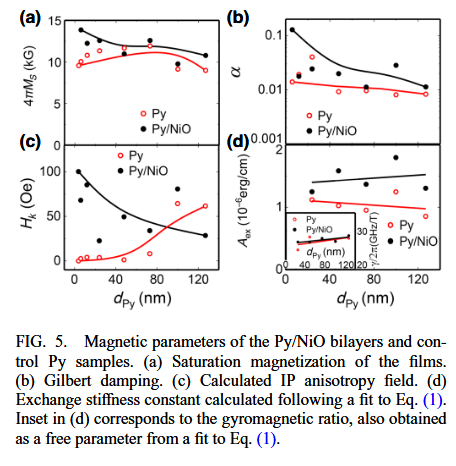
\includegraphics[width=0.65\linewidth]{Images/PSSW_01.png}
            \caption{\textit{Figure from the paper, important one}}
            \label{fig:PSSW_pp1_01}
        \end{figure}
    \end{enumerate}
\end{enumerate}
\subsection*{\underline{Numerical Results of PSSW presence of Py films}}
\begin{enumerate}[1.]
        \item The thickness of the Py films used in the simulation (done by using Mumax$^3$) ranges from 20 nm - 200 nm.
        \item The films are thick enough to accurately resolve the PSSW modes and to observed their possible shifts in the frequency when the interaction with the AFM is introduced.
        \item The surface magnetization gradient caused by a possible oxidation and/or capping, they aim to manipulate the interface pinning parameter, which strongly affects the spin configuration of the PSSW modes across the film \cite{waring2023exchange}.
        \item Not taken in account the surface anisotropies.
        \item Weaker modes above 30 GHz are not observed experimentally in our system due to the strong losses experienced at high frequencies.
        \item In the case of simulation, the detected nodes, $n>0$ are proportional to $1$/$d^2_{Py}$. This agrees with the reports on PSSWs in other FM films.
        \item The frequency of the bulk FMR remains constant when the thickness of the film is increased. Eventually, two modes combine at $d_{Py}< 110$ nm.
\end{enumerate}
\begin{enumerate}[A.]
    \item \underline{Simulating the Py/NiO interface. Optimization of the Uniaxial anisotropy}\\
    The simulations of magnetization dynamics in the AFM-FM bilayer were performed by introducing an extra layer in the system as an uncompensated AFM. This leads to uncompensated spins at the interface, which lead to an exchange bias between FM and AFM.
    \item \underline{Hybrid modes and effect of the interaction with the antiferromagnet}
    \begin{enumerate}[1.]
        \item In both micromagnetics and Atomistic simulations, AFM sublattices are used to model the system \cite{jenkinsAtomisticOriginAthermal2021,jenkinsAtomisticOriginExchange2020}.
        \item Shift in the frequency of the modes, especially in the experimentally observed first-order PSSW $(n=1)$, is also present in all of the performed simulations featuring an AFM-FM interface.
        \item The uniaxial anisotropy at the interface has a direct influence on the frequency of the PSSWs. As given in the diagram, uniaxial anisotropy induced by the AFM leads to higher-frequency modes.
        \item The frequency of the modes can be further enhanced by introducing a local in-plane exchange bias field in the bottom layer of the order of $H_{eb}=1$ kOe. 
    \end{enumerate}
    \item \underline{Conclusion}
    \begin{enumerate}[1.]
        \item They have detected both perpendicular PSSWs spin waves and quasiuniform modes and found that in sufficiently thick Py films both exhibit a clear frequency shift when Py is exchange coupled to NiO.
    \end{enumerate}
\end{enumerate} % 2024 Standing Spin waves in Py/NiO 
% \section{Interfacial Spin Configurations and the Microscopic Origin of Exchange Bias at the IrMn/CoFeB Interface \href{https://doi.org/10.1016/j.fmre.2026.01.003}{[\textit{Fundamental Research, 8 Jan (2026)}]}}

\section*{Main points from the Paper}
\subsection*{\centering\underline{Abstract}}
\hspace{3cm} Exchange bias fields at antiferromagnet/ferromagnet (AFM/FM) interfaces' physical origin remains incompletely understood. While the most of the spins are strongly coupled to the adjacent CoFeB layer, a small fraction remains pinned to the underlying IrMn underlayer. Micromagnetic simulations indicates that an imbalance in the quantity of antiparallel pinned spins contributes to the observed variation in exchange bias.

\subsection*{\centering\underline{I. Introduction}}
\begin{enumerate}
    \item Study of AFM/FM interface has greater impact in the study of spintronics. Exchange bias, being a notably in the AFM/FM structures have a significant in the performance of spintronic devices.
    \item \hl{Exchange bias (EB)} refers to the shift of the magnetization hysteresis loop caused by interfacial coupling between the AFM and FM layers.
    \item EB was generally used to stabilize the magnetization of the pinnned or reference layer in spin-valve structures and MTJs. Moreover, spin-orbit torque (SOT) switching of perpendicular magnetization without an external magnetic field can be realized by introducing an in-plane EB field.
    \item In this work CoFeB/MgO structure provides strong perpendicular magnetic anisotropy and large tunneling magnetoresistance.
    \item Due to the recent development in the electrical control of EB via SOT has been demonstrated, enabling the development of a novel storage prototype known as AFM random-access memory.
    \item Earlier studies  have explained that EB originates from fully uncompensated AFM spins [\textcolor{red}{ref. 39}], planar domain-wall model to reconcile the quantitative discrepancies between theoretical predictions and experimentally measured the EB fields [\textcolor{red}{ref. 40}]. Subsequently, Malozemoff developed the random-field model to account for the influence of interface roughness and defects [\textcolor{red}{ref. 42}].
    \item These established that the coupling between FM spins and pinned AFM  spins is a key microscopic mechanism responsible for the EB field.
    \item Recently, the electrical control of EB via SOT have shown that spin current can partially switch the EB field, this is particularly attributed to the formation of AFM multidomains during manipulation process, suggesting that the orientations of interfacial AFM spins, and their contributions to the exchange bias field, are more complex than previously studied.
    \item X-ray magnetic circular dichroism (XMCD)  is employed as a high-precession technique for probing and analyzing AFM/FM interfaces.
    \item Measurements are taken as;
    \begin{itemize}
        \item XMCD measurements at different temperature is done.
        \item Element-specific XMCD hysteresis loops are measured to determine the orientation of AFM pinned spins in samples annealed under different magnetic fields.
    \end{itemize}
    \item Micromagnetic simulations show that variations in the exchange bias field are primarily governed by the quantitative imbalance between these pinned-spin populations.
\end{enumerate}

\ding{107} \hl{Materials and Methods section is not included in these notes}.
\subsection*{\centering\underline{II. Results and Discussion}}
\begin{enumerate}
    \item The multilayer exhibits perpendicular magnetic anisotropy along with an out-of-plane exchange bias field. They have observed the monotonically increment in the magnitude of the EB with the annealing field and saturates at $\pm1$ T.
    \item 
\end{enumerate} %2026 Paper related to IrMn/CoFeB
% \section{Magnetocrystalline Anisotropy Enables Field-Free Deterministic Switching in $\mathrm{Tm_3Fe_5O_{12}/Pt}$ Bilayers: An Atomistic Spin Dynamics Study - [\href{https://doi.org/10.1021/acsami.5c23180}{\textit{ACS Applied Materials \& Interfaces}, 2026}]}

\section*{Main points from the Paper}
\subsection*{\centering\underline{Abstract}}
\hspace{2cm} Field-free switching of perpendicular magnetization is done in this paper. They have observed that the cubic magnetocrystalline anisotropy (MCA) of TmIG spontaneously breaks mirror symmetry along the out-of-plane direction, giving rise to $\mathrm{3m-}$symmetric torques that enable deterministic switching without external fields. Systematic tuning of current density and pulse width allows control over the switching-mode. They have also done the comparative simulations on $\mathrm{Y_3Fe_5O_{12} (YIG)}$ to confirm that MCA-driven field-free switching is a universal feature of rare-earth iron garnets.

\subsection*{\centering\underline{I. Introduction}}
\begin{enumerate}
    \item Manipulation of perpendicular magnetization by spin-orbit torque (SOT) has recently emerged as the cornerstone for high-density, ultrafast, and energy-efficient spintronic devices.
    \item In the absence of external symmetry breaking, the system relaxes stochastically into up or down states once the current is turned off.
    \item It is usually enforced by an in-plane magnetic field [\textcolor{red}{ref. 1, 2, 6}]
    \item Eliminating the need for external fields requires intrinsic symmetry breaking.
    \item Recently, crystalline symmetry itself has been identified as an intrinsic pathway to deterministic SOT switching, demonstrated low symmetry materials such as $\mathrm{WTe_2, IrO_2, Ni_4W}$ as well as in  noncollinear antiferromagnets and altermagnets.
    \item These systems exploit symmetry-governed spin textures to generate characteristic angular responses in field-free magnetization switching.
    \item Not relying on the structural asymmetry, the effect originates from the intrinsic MCA of TmIG [\textcolor{red}{ref. 34\&35}].
    \item This discovery highlights a fundamentally new mechanism for field-free SOT switching in high-symmetry crystals, relying on intrinsic anisotropy rather than extrinsic structural asymmetry.
    \item They have done the cubic MCA mediated switching across rare-earth iron garnets and done that for both TmIG and YIG.
    \item This work mainly provides the anisotropy-driven spintronic phenomena and establish a symmetry-based design principle for ferrimagnetic memory and terahertz spintronic applications.
\end{enumerate}
%%%%%%%%%%%%%%%%%%%%%%%%%%%%%%%%%%%%%%%%%%%%%%%%%%%%%%%%%%%%%%%%%%%%%
\subsection*{Meeting with Rajnandini about the TmIG, Jan 24, 2026}
We discussed more in details about the TmIG and we both finalized that we need to just go through the paper first and then can later work on designing the material in the VAMPIRE. 

I will work on the understanding of the \verbatiminput{sim:unit-cell-category} part and then only I will work on developing this system.
%%%%%%%%%%%%%%%%%%%%%%%%%%%%%%%%%%%%%%%%%%%%%%%%%%%%%%%%%%%%%%%%%%%%%%%%%
\subsection*{\centering\underline{II. Methods and Materials}}
\begin{enumerate}
    \item $\mathrm{Tm_3Fe5O_{12} (TmIG)}$ is a cubic rare-earth iron garnet  with lattice constant $\sim 12.3$ \r{A} with Fe$^{3+}$ ions occupying octahedral (a-site) and tetrahedral(d-site) positions, while Tm$^{3+}$ ions reside in dodecahedral (c-site) positions.
    \item There is antiferromagnetic coupling between the Fe sublattices and parallel alignment of Tm$^{3+}$ moments with a $a$-site Fe$^{3+}$ sublattice yield a ferrimagnetic ground state with non-zero net magnetization.
    \item Though being TmIG as intrinsic cubical anisotropic, the magneto elastic coupling plays a crucial role in orienting the magnetization in epitaxial TmIG thin films.
    \item Here, they have considered an epitaxial $(111)$-oriented TmIG film capped with a Pt layer.
    \item TmIG being a magnetic insulator, the charge current is limited to the adjacent Pt layer, with TmIG magnetization switching driven by SOT generated from Pt-converted pure spin current injected into TmIG.
    \item The \hl{details of the simulations} are given below:
    \begin{enumerate}[\ding{212}]
        \item The damping parameter used is, $\mathrm{\alpha=0.033}$.
        \item The three-sublattice model $(\mathrm{Fe_1, Fe_2, Tm})$ is used with periodic boundary conditions in the $\mathrm{x-y}$ plane.
        \item The TmIG film is oriented along the $[111]$ axis normal to the plane.
        \item The Hamiltonian only includes the exchange interactions, uniaxial PMA, and MCA terms. [See eqn: 1 of the paper]
        \item The SOT was modeling as a damping-like term, with its amplitude $H_{DL}$ being proportional to the applied current density.
        \item The temperature dependent magnetization curve simulated via the atomistic model has Curie temperature of \hl{$\sim 530$ K}, matching experiments and validating model accuracy.
        \item \hl{See the supporting information again after this to know more about the simulation details}.
    \end{enumerate}
\end{enumerate}
\subsection*{\centering\underline{III. Results and Discussion}}
\subsubsection*{\underline{A. Spin-Orbit Torque Driven Switching}}
\begin{enumerate}
    \item The thickness of the Pt used here is 3nm, and in-plane charge current density is applied which created a pure spin current $j_s$ along $+z$ direction via spin-orbit coupling.
    \item After rotating the direction of $j_c$, the azimuthal angle $\sigma$ denoted by $\Phi_{\sigma}$. The normalized net magnetization, $\sum_i\mu_{s,i}S_i/\sum\mu_{s,i}$ for representative case $(\Phi_{\sigma}=0^\circ, 30^\circ, 90^\circ)$ under a 2 ns charge current pulse (corresponding to a damping-like SOT field $H_{DL}=0.5$ T).
    \item Upon the pulse injection the Magnetization component $\mathrm{M_z}$ dropped to zero within picosecond time $(\sim 11$ ps$)$.
    \item The magnetization reversal was only observed at $(\Phi_{\sigma}= 30^\circ$ and $90^\circ)$ within 5.5 ns whereas, no reversal was seen at $(\Phi_{\sigma}=0^\circ)$.
    \item The switching polarity reverses every $60^\circ$, manifesting the intrinsic 3-fold angular periodicity of TmIG. And this periodicity originates from the material's MCA, which generate as effective anisotropy field proportional to $\sin3\Phi_{\sigma}$.
    \item At each of these critical angles $(\Phi_{\sigma}=n\cdot60^\circ, \mathrm{where}$ $n = 0, 1, ...,6)$, the MCA contribution vanished, which restores pure PMA symmetry and yields equal probabilities for up and down states.
    \item In order to get the microscopic origin of the field-free switching, they have analyzed the spin torques during the relaxation dynamics.
    \item Once current pulse is turned off $t=2.5$ ns $)$, the SOT contribution vanished, and the spin evolution is governed solely by the intrinsic torque $\mu_{s,i}\mathrm{S}_i\times\mathrm{H_{eff}^i}$, where the local effective field $\mathrm{H_{eff}^i}$ includes local Heisenberg exchange interactions and MCA contributions.
    \item The net magnetization $\mathrm{\textbf{M}}$ is locked along $[1\bar10]$. The thermal fluctuations can destabilize this state, leading ot stochastic relaxation toward either the $+z$ or $-z$ orientation.
    \item When the $\Phi_{\sigma}=30^\circ$ ($\sigma||[2\overline{11}]$), the MCA field generates finite torque despite vanishing contributions from PMA and exchange. This torque is responsible for the magnetization precession and ultimately forces relaxation toward a new equilibrium state along $-z$.
    \item Further the effect of the SOT on the amplitude of magnetization reversal by applying 5 ns current pulses was also studied.
    \item A critical threshold of SOT field $(\sim 0.9$ mT$)$ is identified. Below this value, the magnetic moment only tilts slightly from its initial $+z$ orientation and relaxes back after the pulse.
    \item And above this threshold, the magnetization is driven into the in-plane direction defined by $\sigma$, enabling deterministic reversal to $-z$.
    \item While the PMA remains isotropic in the xy-plane and the exchange field sows negligible angular dependence, the MCA exhibits a distinct 3-fold rotational symmetry.
\end{enumerate}
\subsubsection*{\underline{B. THz Oscillations and Toggle-Like Switching}}
\begin{enumerate}
    \item High SOT field drives TmIG into a precessional regime making the stabilization of the symmetric switching.
    \item Above the threshold SOT of 3.75 T $(\mathrm{J_c=5.919\times10^{13} A/m^2})$, oscilaltions grow and stabilizes into large-angle precession in a plane perpendicular to $\sigma$.
    \item There is antiphase precession in $Fe_1$ and $Fe_2$ due to the antiferromagnetic coupling, while Tm remains weakly coupled, exhibiting smaller amplitude precession in phase with Fe$_2$.
    \item These three sublattices oscillate at the identical frequency of 3.3954 THz. The oscillation frequency increases linearly with the applied SOT field strength, in agreement with earlier reports. [\textcolor{red}{ref. 46 \& 47}]
    \item This highlight the application of TmIG for high-frequency spnitronic applications.
    \item As the SOT field increases (Fig. 4a), the enhanced oscillations of the z-component magnetization broaden the precessional motion during the pulse, causing the sublattices at the end of the pulse to exit the $M_z=0$ plane and relax stochastically into either the $+z$ or $-z$ state in a non-deterministic manner.
    \item This precession-mediated process enables toggle-like switching in TmIG at high charge-current pulses and a fixed spin polarization $\Phi_\sigma$.
    \item There is contrary switching in the case of Fe$_2$ switching with a 4.2T SOT field, as it relaxes back to the $+z$ direction (parallel to its initial state). This anomalous polarity reversal confirms the toggle-like switching phenomenon in TmIG.
    \item With the constant SOT field of 4.0T but variation in the pulse-width, the toggle-like switching is observed specifically at 7.0 and 8.5 nm, while other durations yield conventional $-z$ switching.
    \item These results demonstrate that the combined control of current density and pulse width provides a pathway to modulate switching modes in TmIG/Pt devices, bridging deterministic to toggle-like switching regimes.
    \item This helps for high density "SOT-MRAM" for reliable "write-erase" cycling.
\end{enumerate}
\subsubsection*{\underline{C. Generalization of 3m-symmetry SOT Switching In Rare-Earth Iron Garnets}}
\begin{enumerate}
    \item They have also performed these calculations on $\mathrm{YIG, Y_3Fe_5O_{12}}$, which shares the TmIG's crystal structure and exhibits both MCA and PMA due to magnetoelastic coupling.
    \item  2 ns current pulses with an effective SOT field of 0.5 T at varying azimuthal angles, YIG exhibits a $3m$-symmetric switching behavior analogous to TmIG.
    \item The low damping constant in the case of TIG prolongs the relaxation time.
    \item YIG with a lower damping constant shows smoother magnetization dynamics and reduced post switching oscillations, which can facilitate faster and more stable switching.
    \item The switching performance in the YIG originates from the lower MCA energy of YIG, which results in more isotropic in-plane magnetic anisotropy, thereby suppressing the MCA-induced $M_z$ wiggles.
    \item Additionally, we have seen that the reduced MCA smooths the switching profile, while PMA variation has minimal effect.
    \item These calculations demonstrate that $3m$-symmetric SOT switching is intrinsic to rare-earth iron garnets and tunable via magnetic anisotropy engineering.
\end{enumerate}
\subsection*{\centering\underline{IV. Conclusion}}
Atomistic spin-dynamics simulations show that TmIG/Pt bilayers can achieve deterministic, field-free magnetization reversal driven by spin-orbit torque, with a characteristic threefold angular symmetry set by cubic magnetocrystalline anisotropy. At low current densities, the switching threshold varies periodically with the in-plane spin-polarization direction, while strong current pulses excite terahertz precession that enables toggle-type switching controlled by pulse width. Similar behavior is found in YIG, with faster dynamics. Overall, materials combining MCA and perpendicular anisotropy provide a symmetry-based route to low-power spintronic switching, though thermal effects from high currents remain to be addressed in future work.

\hl{See the supporting information in ZoTeRo for the parameters and then do follow this writing here.} % Very recent ASD paper of TmIG
% \section{Atomistic study of Positive Exchange Bias in Hard/Soft ferromagnetic bilayer nanosystem \href{https://doi.org/10.1088/1402-4896/acb23c}{[\textit{Physica Scripta, 98 2 025403 (2023)}]}}


\section*{Main points from the Paper}
\subsection*{\centering\underline{Abstract}}
\hspace{2cm} The calculations for the exchange spring nano-bilayer with intermixing of high and low anisotropic moments at the interface are studied in this paper, and an unexpected phenomenon of positive exchange bias is observed. \hl{The influence of temperature is clearly observed in the shift and the width of the M-H loop}. They have claimed that the interface roughness is the main cause for the shift in the hysteresis loop.    
\subsection*{\underline{I. Introduction}}
\begin{enumerate}
    \item The multilayer exhibits perpendicular magnetic anisotropy along with an out-of-plane exchange bias field. They have observed a monotonically increasing EB magnitude with the annealing field, which saturates at $\pm1$ T.
    \item The exchange-bias effect was seen first in the core-shell structure, and later, this was also observed for the FM-AFM system.
    \item The coupling between FM and AFM spins at the interface adds an internal field (bias field) to the applied field, which is a trivial source of asymmetrical hysteresis loop and eventually leads to the existence of exchange bias. 
    \item Also, the induction of anisotropy at the interface might be another reason for the unidirectional shift of the loop. [\textcolor{red}{ref. 4 -anisotropy affects the EB}]
    \item Exchange bias is commonly used in magnetic sensors due to the enhanced thermal stability of the material; other technological applications include GMR devices, hard disks, and hard drives, and it also serves as the basis for many other applications in spintronics.
    \item Of many existing theoretical assumptions for the exchange bias, one of the main ones is the presence of interfacial uncompensated AFM spin magnetic moments [\textcolor{red}{ref.9: Exchange Bias paper.}]
    \item Different morphology systems have been studied for EB-related studies, mostly done for the thin film bilayers, as there can be enhanced control over the interface, and they are more suitable for device fabrication.
    \item The shift in the M-H loop can be in any direction.
    \item Positive EB is far less common than negative EB as found in several heterostructures.
    \item The presence of AFM exchange coupling at the interface of the FM bilayer system is responsible for the EB effect. 
    \item A large amount of disorder present at the interface of the FM-AFM can also be the reason for this effect.
    \item Atomistic spin models are used to study the exchange-bias field caused by the roughness in simple cubic Co/CoO core-shell NPs \cite{wuInfluenceAtomicRoughness2020,influenceofinterfacial2011}. 
    \item A key feature of the exchange bias effect, i.e., unidirectional shift of the hysteresis loop, is observed.
\end{enumerate}

\subsection*{\underline{II. Methods}}
\begin{enumerate}
    \item Classical Heisenberg Hamiltonian and Landau-Lifshitz Gilbert equations are employed to study the EB effect in Hard/Soft FM Fe/Co bilayers.
    \item Both flat and roughened surfaces are simulated, particularly looking for the effect of roughness on the EB.
    \item Details about the system for the simulation and system are:
    \begin{enumerate} [\ding{212}]
        \item BCC crystal structure for both Fe and Co.
        \item Dimension of the system: $x=10$ nm, $\times y=10$ nm, $\times z=4$ nm. total atoms, 32368 atoms with $50\%$ Fe and $50\%$ Co.
        \item Understand the extensively written Hamiltonian.
        \item Exchange interactions: {$J_{Co}=-6.064\times10^{-21}J/link$}; \\{$J_{Fe}=-7.05\times10^{-21}J/link$}; {$J_{Fe-Co}=1.0\times10^{-22}J/link$}
        \item Uniaxial anisotropy: {$K_{Co}=6.69\times10^{-24}J/atom$}; \\{$K_{Fe}=5.65\times10^{-25}J/atom$}
        \begin{table}
            \centering
            \begin{tabular}{ccccc}\hline \hline
                Symbol & Value & Parameter & Units & \\ \hline 
                $\alpha$ &  & Gilbert Damping paramter  & - & \\
                 &  &  &  & \\
                 &  &  &  & \\
                 &  &  &  & \\
                 &  &  &  & \\
                 &  &  &  & \\ \hline \hline
            \end{tabular} 
            \caption{Parameters used for the Exchange bias calculation for the Fe/Co in Junaid Ahsan's paper}
            \label{tab:Fe/Co_parameter_EB}
        \end{table}
        \item Uniaxial anisotropy direction = 0, 0, 1 for Co and 1, 0, 0 for Fe.
        \item Heun integration scheme was used for the hysteresis calculations.
        \item Here for the easy damping, the critical damping value is used; $\alpha=1.0$ [\textcolor{red}{19, 20}]
        \item Applied field was varied from: $+1.0$ T to $-1.0$ T in steps of $0.001$ T.
        \item The magnetic field was applied along the $xy-plane$ of the bilayer.
        \item The details of time-steps are;
        \begin{verbatim}
            equilibration-time-steps=100000
            loop-time-steps=100000
        \end{verbatim}   
    \end{enumerate}
\end{enumerate}

\subsection*{\underline{III. Results and Discussions}}
\begin{enumerate}
    \item The influence of interface roughness was studied by Evans et.al.,\cite{influenceofinterfacial2011} for FM-AFM core-shell spherical nanoparticles. The roughness gives rise to uncompensated magnetic moments at the interface. 
    \item The degree of coupling between the FM and AFM was increased by the roughness at the interface. 
    \item EB fundamentally being an interfacial phenomenon, any modification of the interface structure has a significant effect on it.
    \item The change in the microstructure in the different crystalline orientations changes due to intermixing of hard and soft atomic spin moments.
    \item Additionally, the other prerequisite for EB is that there is a difference in the anisotropy of two catenated layers; if not, then they will rotate under the effect of an externally applied field coherently.
    \item In this paper, the shape of the M-H loop is decided by the direction of the applied field and the magnetic anisotropy in the Fe and Co.
    \item The uniaxial anisotropy direction is set as per the easy axes of the individual system. For Fe, it is 100; for Co, it is 001. This is the case for a bulk system.
    \item If the anisotropy is along the same direction, then one would expect a more square loop.
    \item There is a difference in the magnitude and also the direction of the anisotropy in this paper for observing the Positive EB (PEB).
    \item There is a shift in a positive direction in all of the cases when the interface is flat, i.e., there is no intermixing.
    \item The positive EB in the smooth interfaced bilayer can thus be attributed to the;
    \begin{itemize}
        \item larger magnetic anisotropy energy of the hard (Co) layer than the soft (Fe) layer.
        \item ferrimagnetic nature of the interface.
        \item anisotropy direction.
    \end{itemize}
    \item The alloy formation at the interface leads to the enhancement in the EB as observed in all simulated temperatures.
    \item There is a decrease in the coercivity with elevating temperature.
\end{enumerate}

\subsection*{\underline{IV. Conclusions and further work}}
\begin{enumerate}
    \item Positive EB was studied using ASD, with AFM coupled Fe/Co magnetic bilayer system.
    \item It is verified that EB is an interfacial phenomenon.
    \item Major contribution comes from the interfacial exchange interaction between Co and Fe magnetic spin moments.
    \item Improvements in the positive EB were observed after increasing the roughness.
\end{enumerate}
\vspace{1cm}
The effect of EB variation on the degree of roughness and interfacial mixing of atomic moments can be studied. - \hl{Future Work Related} % 2023-Atomistic paper for EB related work_ Junaid_01
% \newpage
\section{Exchange bias study in FM/AFM bilayers: Atomistic simulations \href{https://doi.org/10.1016/j.physo.2025.100265}{[\textit{Physics Open, 23 April (2025)}]}}


\section*{Main points from the Paper}
\subsection*{\centering\underline{Abstract}}
\hspace{2cm} The study of exchange bias (EB) effect through simulations is done by utilizing the LLG equation and Heisenberg Spin model Hamiltonian for FM/AFM bilayer system. The AFM layer near the interface was disturbed, and the bilayer's M-H loop broadened and became asymmetric.
The EB effect can be artificially tuned by adjusting the heterostructure, which can be useful for scientific applications.


\subsection*{\underline{I. Introduction}}
\begin{enumerate}
    \item The shift in the hysteresis loop when a magnetic system is composed of a ferromagnetic(FM) and antiferromagnetic(AFM) layer. This is the numerical shift of the M-H loop.
    \item The modulus of the average of the difference between the positive $H_c(+ve)$ and negative $H_c(-ve)$ coercive field, if positive, is the numerical value.
    \item The EB has been observed in various systems, ferrimagnets (FI), spin glass(SG), and spin disorder (SD).
    \item The geometries like core-shell, bilayers, and multilayers have been studied to study the EB effect because the interface can be easily tuned in these systems.
    \item The phenomenon of EB is a direct consequence of the exchange interaction between two differently ordered magnetic layers at their interface.
    \item Some factors that affect the EB strength directly are:
    \begin{itemize}
        \item strength of the exchange coupling,
        \item thickness of differently ordered magnetic layers,
        \item temperature of the system.
    \end{itemize}
    \item The exact behavior of $H_{eb}$ as a function of temperature can vary depending on the specific materials, magnetic ordering, and nature of the interface.[\textcolor{red}{ref. 7-9, very imp.}]
    \item They have done Atomistic spin dynamics simulations for Cobalt(Co) \& AFM (CoO) in the framework of classical spin Hamiltonian and LLG equation.
    \item ASD simulations are immensely useful in determining temperature-dependent magnetic properties.
    \item The hysteresis provides a lot of information about the magnetic properties of the system. In this case, the loops are simulated with flat and roughed interfaces between FM/AFM layers.
    \item Interface mixing is central to the method in this system.
    \item This work demonstrates that controlled interfacial intermixing of FM spins within the AFM layer directly affects the M-H loop.
    \item The systematic integration of FM moments into the AFM bulk suggests that EB can be tailored by adjusting the spatial distribution of uncompensated moments.
\end{enumerate}

\subsection*{\underline{II. Methods}}
\begin{enumerate}
    \item Details about the system for the simulation and system are:
    \begin{enumerate} [\ding{212}]
        \item BCC crystal structure for both Co and CoO.
        \item Dimension of the system: $x=2$ nm, $\times y=2$ nm, $\times z=6$ nm. total atoms, 2448 atoms with $70\%$ Co and $30\%$ CoO.
        \item Understand the extensively written Hamiltonian.
        \item Exchange interactions: {$J_{Co}=6.064\times10^{-21}J/link$}; \\{$J_{CoO}=-4.21\times10^{-21}J/link$}; {$J_{Co-CoO}=5.6\times10^{-22}J/link$}
        \item Uniaxial anisotropy: {$K_{Co}=4.644\times10^{-24}J/atom$}; \\{$K_{CoO}=4.644\times10^{-23}J/atom$}
        \item Magnetic moments are: $\mu_{Co}=1.72\mu_B$ and $\mu_{CoO}=3.5\mu_B$ 
        % \begin{table}[h!]
        %     \centering
        %     \begin{tabular}{ccccc}\hline \hline
        %         Symbol & Value & Parameter & Units & \\ \hline 
        %         $\alpha$ &  & Gilbert Damping paramter  & - & \\
        %          &  &  &  & \\
        %          &  &  &  & \\
        %          &  &  &  & \\
        %          &  &  &  & \\
        %          &  &  &  & \\ \hline \hline
        %     \end{tabular} 
        %     \caption{Parameters used for the Exchange bias calculation for the Fe/Co in Junaid Ahsan's paper}
        %     \label{tab:Fe/Co_parameter_EB}
        % \end{table}
    %     \item Uniaxial anisotropy direction = 0, 0, 1 for Co and 1, 0, 0 for Fe.
        \item Heun integration scheme was used for the hysteresis calculations.
    %     \item Here for the easy damping, the critical damping value is used; $\alpha=1.0$ [\textcolor{red}{19, 20}]
        \item Applied field was varied from: $+1.0$ T to $-1.0$ T in steps of $0.001$ T.
    %     \item The magnetic field was applied along the $xy-plane$ of the bilayer.
        \item The details of time-steps are;
        \begin{verbatim}
            equilibration-time-steps=100000
            loop-time-steps=100000
            time-step = 1.0e-15
        \end{verbatim}   
    \end{enumerate}
    \item The LLG equation models the fact that spin moments in a ferromagnet do not align with the local field direction. Instead, they undergo precession under the influence of an external magnetic field.
    \item The precession cannot continue indefinitely, as it is damped.
    \item Microscopic damping is denoted by $\alpha$. In this paper, they have used $\alpha=1.0$ as the critical damping.
\end{enumerate}

\subsection*{\underline{III. Results and Discussions}}
\begin{enumerate}
    \item Exchange bias (EB) is basically a shift in the magnetic hysteresis loop $(H_{\mathrm{EB}})$ and alterations in its coercive width $(H_{\mathrm{C}})$.
    \item Previous studies have emphasized the role of cooling fields in establishing EB--where higher fields reduce $(H_{\mathrm{EB}})$ and may even induce positive bias [\textcolor{red}{ref. 25}]
    \item The approach used in this work is to initialize the FM and AFM layers in the magnetization state expected at the end of the cooling process.
    \item And the simulation temperature remains well below the N\'eel temperature, which helps in preserving the magnetic order while eliminating the need for external cooling fields.    
    \item The temperatures at which the simulations are conducted are 0 K, 5 K, and 10 K, which exhibit perfect symmetry about the field axis, confirming the absence of EB in fully compensated systems.
    \item Introducing the controlled interfacial uncompensated through FM-AFM intermixing dramatically alters this behavior.
    \item The intermixing parameter of 0.07 is used in this work. Here, the FM moments penetrate the AFM bulk.
    \item This subtle modification generates localized spin frustration, disrupting AFM exchange interactions and creating a net interfacial magnetization.
    \item This is as observed in the case of spin-glass dynamics in partially disordered AFM layers \textcolor{red}{[28,29]} where low FM doping near the interface creates localized frustration.
    \item And as a result, the broadening of the hysteresis loops is observed, which is attributed to the increasing energy barrier for magnetization switching.
    \item The significantly observed EB values are: 53 mT, 46 mT, and 28 mT at 0 K, 5 K, and 10 K, respectively.
    \item Any M-H loop with temperature greater than 10 K, the simulated loops were very noisy due to the thermal fluctuations of the atomic spin moments and in adequate to furnish any physical results.
    \item At zero field, intermixed FM moments induce spin canting (frustration) within the AFM lattice, creating an uncompensated interface.
    \item The application of $-1.0$ T field aligns FM moments antiparallel to the field while pinning AFM spins through exchange coupling.
    \item As the field reverses to $+1.0$ T, the FM layer rotates coherently, overcoming the unidirectional anisotropy imposed by the disordered AFM interface.
    \item This asymmetry in the magnetization reversal route directly produces the observed EB \cite{influenceofinterfacial2011}, rather than bulk anisotropy-- a conclusion our intermixing approach corroborates while extending to controlled doping scenarios.
    \item The straight $47\%$ reduction in $H_{\mathrm{EB}}$ from 0 K to 10 K reflects thermal disruption of interfacial coupling, while parallel $43\%$ $H_C$ decrease indicates reduced domain stability.
    \item The temperature sensitivity of EB $(\Delta H_{\mathrm{EB}}\approx-2.5$ mT/K $)$ highlights the need for materials with high $T_N$ and engineered interfaces to sustain functionality across operational temperature ranges.
    \item Furthermore, enhancing EB through controlled uncompensation while reducing thermal stability suggests optimal doping level exists for specific applications.
    \subsubsection*{Effect of ferromagnetic layer thickness on exchange bias}
    \item Since EB is primarily an interfacial effect, if the thickness of the FM layer is increased, the same interface pinning force has to affect a large volume of the FM, effectively diluting its impact and reducing the effective EB field. Empirically, $H_{\mathrm{EB}}\propto\frac{1}{t_{FM}}$, confirming that as the thickness of the FM layer increases, the overall effect of the interfacial pinning diminishes.
    \item Three cases where the FM thickness is 0.7 t, 0.75t, and 0.80t at 0 K are plotted, and the M-H loop area is diminished significantly.
\end{enumerate}

\subsection*{\underline{IV. Conclusions and Further work}}
\begin{enumerate}
    \item This work demonstrates that the EB in the FM/AFM bilayer system can be well controlled through the interfacial intermixing of FM spins into the AFM layer.
    \item With the help of ASD, it has been shown that the spatial distribution of uncompensated AFM moments plays a vital role in the manifestation of EB.
    \item The direct correlation between FM intermixing, EB behavior, broadening of M-H loop, and thermal effects, such as blocking temperature, is observed in this paper.
    \item This study provides insights into how interfacial modifications influence macroscopic EB properties, emphasizing the importance of microscopic spin interactions in determining macroscopic behavior.
\end{enumerate} %2025-Atomistic paper for EB related work_ Junaid_02
\section{Excitation and modulation of exchange spin waves in CoFeB films \href{https://doi.org/10.1063/5.0169995}{[\textit{Appl. Phys. Lett., 123 172402 (2023)}]}}


\subsection*{\underline{Abstract}}
The excitation and modulation of the spin waves in $\mathrm{Co_{20}Fe_{60}B_{20}} (\mathrm{CoFeB})$ films by varying magnetic anisotropy. The film thickness is 50 nm. The effective excitation PSSW is achieved due to the uniaxial anisotropy induced by \hl{oblique scattering sputtering method}. Additionally, the periodic array of rectangles enables excitation of both exchange-dominated surface spin waves and PSSWs, achieved by modulating the rectangle's length-to-width ratio. It is worth noting that PSSWs are present along the easy axis, whereas surface spin waves are observed along the hard axis, highlighting the significant influence of shape anisotropy on spin waves.

\subsection*{\underline{Introduction}}
\begin{enumerate}
    \item There are several advantages of spintronic devices over existing charge-based electronic devices, including joule heating, which is among the most important.
    \item The advantages of devices based on spin waves are;
    \begin{itemize}
        \item Low power consumption.
        \item Fast information processing speed, 
        \item Non-volatility of the system.
        \item Serving as the next generation of information carriers for transmitting and processing data.
    \end{itemize}
    \item Exchange spin waves (ESWs) are short-wavelength spin waves whose dispersion is primarily governed by the exchange interaction, encompassing perpendicular standing spin waves (PSSWs) and exchange surface spin-waves.
    \item The strong interlayer exchange coupling results in lare anticrossing gaps between kittel mode and the high-frequency ESWs. This phenomenon has been observed in various systems, such as YIG/Co, YIG/Py bilayers, and hybrid structure consisting of YIG thin film and nickel nanowires.
    \item Several methods to excite the ESWs are previously studied;
    \begin{itemize}
        \item Spin-torque excitation, 
        \item Utilization of nanoscale magnetic gratings, 
        \item Influence of nonuniform composition [\textcolor{red}{ref. 15}].
    \end{itemize}
    \item If ESWs can be excited in magnetic metal thin films, it would be beneficial for the preparation and development of high-frequency spintronic devices.
    \item Under uniform microwave magnetic fields, the pinning of the magnetic moment in the film contributes to the excitation of ESWs [\textcolor{red}{ref. 17-20}].
    \item The magnetic anisotropy plays an important role in the pinning of the film magnetization [\textcolor{red}{ref. 21-23}].
    \item The oblique sputtering improves the excitation efficiency of PSSWs.
    \item The relative amplitude of generated surface spin waves is found to be correlated with varying length-width ratios of the rectangles which they have designed as a periodic array.
    \item Furthermore, in the case of CoFeB/PMN-PT heterostructure, electric field is utilized to manipulates the resonance field of the PSSW due to the excellent piezoelectronic properties of PMN-PT.
    \item The oblique sputtering induced in-plane uniaxial magnetic anisotropy in the films.
\end{enumerate}

\subsection*{\underline{II. Discussion}}
\begin{enumerate}
    \item The excitation of PSSW generally requires either non-uniform magnetic parameters along the film thickness or surface spin pinning [\textcolor{red}{ref. 27}].
    \item Volume inhomogeneity model also explains the existence of the PSSW.
    \item The oblique sputtering used in this experiment exhibit uniaxial anisotropy, as confirmed by the magnetic hysteresis loop.
    \item The uniaxial magnetic anisotropy of the sample makes the magnetic moment more inclined to be pinned along the easy axis.
    \item As it is well known that the excitation of the PSSW is also influenced by the confined geometry, implying that modifying the boundary conditions of the sample geometry could have an impact on the surface spin pinning.
    \item Hence, the influence of varying shape anisotropy on spin waves is investigated.
    \item The magnetic hysteresis loops of the three samples, it is evident that their anisotropy differs.
    \item The frequency of PSSW is related to the anisotropic field $H_k$, while the variation in the length-width ratio influences shape anisotropy of the sample.
    \item The resonance field of the spin wave mode is higher than that of the uniform precession mode when the magnetic field rotates to the direction of the hard axis.
    \item 
\end{enumerate} % 
\section{Magnetization dynamic of a $\mathrm{CoFe/Co_2MnSi}$ magnetic bilayer structure\href{https://doi.org/10.1063/5.0128519}{[\textit{J. Appl. Phys., 133 093902 (2023)}]}}


\subsection*{\underline{Abstract}}
Magnetization dynamics of a thin epitaxial $\mathrm{Co_2MnSi(CMS)}$ in magnetic $\mathrm{CoFe/CMS}$ bilayer structured sputtered on MgO substrate is studied. Fourfold symmetry with respect to the azimuthal applied field angle was obtained as the frequency response of the magnetization precession of $\mathrm{CoFe/CMS}$. Moreover, the effective Gilbert damping $\alpha_{\mathrm{eff}}$ exhibits inhomogeneous broadening at lower applied magnetic fields. And at large fields, the azimuthal angle dependence disappears, and the intrinsic damping is observed. 

\subsection*{\underline{I. Introduction}}
\begin{enumerate}
    \item Due to the epitaxial growth of magnetic multi-layers, precise control of electronic and magnetic properties for applications such as magnetic random access memory (MRAM), sensors, and spin transistors is possible.
    \item These devices rely mostly on the multi-layer magnetic tunnel junctions (MTJs), in which high spin polarization is essential to maximize the TMR, and end up optimizing the efficiency of the whole system.
    \item Heusler alloys are coming up as very promising candidates because of the following reasons;
    \begin{itemize}
        \item Half-metallic nature,
        \item High Curie temperature, and 
        \item particularly $\mathrm{CMS}$ being one of the most promising as it can crystallize in the ordered $L\mathrm{2_1}$ crystal structure, as theoretically it has been shown to possess zero spin down DOS at the Fermi energy.
        \item Excellent static behavior with a TMR ratio of $570\%$ at low temperature and $753\%$ in $\mathrm{CMS/MgO/CoFe}$ structure.
        \item In MTJ applications, Heusler alloys are also promising materials for THz emitters [\textcolor{red}{ref. 28,29}].
    \end{itemize}
    \item Understanding the dynamic properties provides time-dependent device behavior and can reveal important material parameters, such as the Gilbert damping parameter $\mathrm{\alpha_{eff}}$.
    \item And the lowering of the damping in the case of $\mathrm{Co_2FeAl(CFA)}$ and  $\mathrm{Co_2MnSi(CMS)}$ leads to the suppression of the spin-flip processes.
    \item The measurement of the precession frequency of the CMS film at low applied magnetic fields (below 1kOe) and as a function of the azimuthal angle $\phi$ between the applied field and the [110] crystalline direction of the film.
    \item A fourfold symmetric dependence of both the precession frequency and damping as a function of $\phi$ was observed, caused by the magnetocrystalline anisotropy present in this cubic structure.
    \item Using various magnetic fields applied at various polar and azimuthal angles, they have extracted the magnetization dynamics all the way up to the high-field limit, where inhomogeneous broadening mechanisms disappear, and intrinsic Gilbert damping of the material can be determined.
    \item \hl{Additionally, it has been found that the angular dependence of the damping parameter disappears in the high magnetic field}.
\end{enumerate}

\subsection*{\underline{II. Sample and Experimental Procedure}}
\begin{enumerate}
    \item Two different samples, $\mathrm{Co_{50}Fe_{50}}$ film was prepared on MgO[001] substrate, and the second sample consisted on a CoFe(1.7 nm)/CMS (7.0 nm) bilayer film.
    \item The layer thickness of the CoFe/CMS bilayer film was determined from X-ray reflectivity, and 1.7 nm CoFe and 7.0 nm CMS were recorded with sharp interfaces of \hl{0.3 nm roughness}.
    \item The bulk CMS compound has a \hl{lattice constant of 0.5654 nm} [\textcolor{red}{ref. 39}].
    \item Magnetization dynamics were analyzed using a dual-color time-resolved magneto-optic Kerr effect (TR-MOKE) setup in polar Kerr geometry.
    \item As the pump beam is spectrally filtered after the reflection, the collected signals provide information on the change in polarization due to the magnetization dynamics.
\end{enumerate}
\subsection*{\underline{III. Results and Discussion}}
\begin{enumerate}
    \item The magnetization dynamics of the epitaxial CoFe were first analyzed, with an external magnetic field of $\mathrm{H_{app}=5}$ kOe applied at multiple polar angles $(\theta,$ angle with respect to the z-axis$)$ and various azimuthal angles $(\phi,$ angle with respect to the x-axis in the $x-y$ plane$)$.
    \item The fourfold symmetry in the BCC structure was probed particularly at polar angles of $\theta=30^\circ,45^\circ,$ and $55^\circ$, and the azimuthal angle was scanned in each case between $0^\circ \leq \phi\leq 90^\circ$ to probe the full fourfold symmetry in the BCC structure.
    \item The dependence of the magnetization precession as a function of azimuthal angles is obtained for three different polar angles.
    \item The effective damping parameter was highest when the in-plane component of the magnetic field was applied along the hard axis $(\phi=0^\circ, 90^\circ)$ and lowest when the in-plane component of the magnetic field was applied along the easy axis  $(\phi=45^\circ)$. [\textcolor{blue}{Important line}]
    \item In the case of the single-layer CoFe film, the frequency response was symmetrically centered around $\phi=45^\circ$.
    \item The azimuthal scan now shows a frequency maximum when the in-plane component of the magnetic field was applied along the $\langle110\rangle$ direction and a minimum along the $\langle100\rangle$.
    \item The field-dependent effective damping parameter was extracted by fitting the data using $\theta_k=A \sin(\omega t+\varphi)e^{-t/\tau}$, $\omega=2\pi f$
    \item In this CMS film, two-magnon scattering (TMS), e.g., due to strain-induced anisotropy inhomogeneities, is a dominant source of extrinsic damping.
    \item At low fields, the apparent difference in $\mathrm{\alpha_{eff}}$ as the azimuthal angle is varied, while the high-field limit appears uniform for all orientations.
    \item The clear dependence of $\mathrm{\alpha_{eff}}$ on $\phi$ was observed with maximum damping at $\phi=45^\circ$, in agreement with the observations of Liu $et$ al. where the inhomogeneous broadening explains the magnetocrystalline anisotropy.
    \item At high applied fields, however, this dependence disappears, and the intrinsic Gilbert damping of $\sim 0.02$ is observed for all parameter combinations.
    \item We note that the relatively $\mathrm{\alpha_{eff}}$ may be due to the mechanical strains present in both the very thin CoFe and the CMS films.
    \item And these strains create defects in the crystal which cause additional spin wave scattering, leading to a larger effective damping parameter $\mathrm{\alpha_{eff}}$.
\end{enumerate}
 % CoFe/Co2MnSi related paper
\section{Field and fluence dependences of laser-induced multiple spin-wave dynamics in $\mathrm{Co_2FeAl_{0.5}Si_{0.5}}$ films \href{https://doi.org/10.1063/5.0006321}{[\textit{J. Appl. Phys., 127 233903 (2020)}]}}


\subsection*{\underline{Abstract}}
Field and fluence-dependent spin-wave dynamics of a full-Heusler $\mathrm{Co_2FeAl_{0.5}Si_{0.5}}$ film studied by using TR-MOKE. Volumetric magnetostatic spin-wave (VMSW) and perpendicular standing spin-wave (PSSW) modes are excited in the films with thicknesses of 60 and 100 nm. Only Kittel mode is observed in the films of thicknesses of 150 and 200 nm. The amplitude of all spin-waves increased with increasing field and fluence and frequency slightly decrease with increasing fluence as expected. Effective damping and lifetimes are both modulated by both external field and excitation fluence. This changes are attributed to the field-dependent group velocity and magnetic inhomogeneity. The dominant mechanism of the electron-phonon scattering enhancement might be the reason for the increment of the effective damping with increasing fluence.

\subsection*{\underline{I. Introduction}}
\begin{enumerate}
    \item Cobalt based heusler/alloys exhibit strong application potentials for magnonic technologies.
    \begin{itemize}
        \item High spin polarization.
        \item Low intrinsic magnetic damping.
        \item Possibility of exciting multiple spin-wave modes (SWMs).
    \end{itemize}
    \item Different spin waves including uniform spin wave (Kittel mode), magnetostatic surface spin-wave (Damon-Eshback (DE) mode), volume magnetostatic spin wave (VMSW), and perpendicular standing spin wave (PSSW) were coherently excited and identified in different cobalt-based Heusler alloy films.
    \item The field-and fluence-dependent spin wave dynamics in full-Heusler $\mathrm{Co_2FeAl_{0.5}Si_{0.5}}$ films with different thicknesses by using TR-MOKE experimental setup with an out-of-plane external field applied.
    \item The VMSW and PSSW modes were excited in two thinner samples, while in the two thicker samples only the Kittel mode is excited.
\end{enumerate}

\subsection*{\underline{II. Experiments}}
\begin{enumerate}
    \item Magnetic sputtering was used to deposit the CoFeAlSi sample on the glass substrate.
    \item The thickness of the sample is 60, 100, 150, and 200 nm.
    \item All the made samples have in-plane magnetized feature that can be attributed to the demagnetizing field.
    \item Pump-probe was used to understand the spin-wave dynamics.
    \item A variable magnetic field generated by an electromagnet is applied along the direction of $\sim 10^\circ$ with respect to the normal of the sample plane.
    \item A nearly perpendicular orientation of the external field is beneficial to create a large precession angle after laser pumping and excite additional SWMs for in-plane magnetized samples [\textcolor{red}{ref. 21}].
    \item All measurements are performed at room temperature $[\mathrm{\sim300 K}]$.
\end{enumerate}
\subsection*{\underline{III. Results and Discussions}}
\subsubsection*{A. Spin-wave dynamics and dispersion analysis}
\begin{enumerate}
    \item The precession of magnetization is launched by the torque exerted on it as the femtosecond pump pulse changes the orientation of the effective field transiently [\textcolor{red}{ref. 19}].
    \item Oscillations with large amplitude with respect to demagnetization indicate the efficient excitation of spin waves.
    \item The Fast Fourier Transform (FFT) spectra of the oscillatory components of the dynamics are obtained and it clearly showed the existence of the spin-waves for 60 nm and 100 nm thickness.
    \item The FFT spectra clearly indicate two different SWMs in the 60 and 100 nm samples but only one SWM in the 150 and 200 nm samples is excited.
    \item The dispersion analysis was also performed to identify the excited SWMs.
    \item Competition between the out-of-plane external field and the demagnetization field results in the slant orientation of the equilibrium effective field.
    \item For the SWM (Kittel mode), the dispersion equation is written as;
    \begin{gather}
        \mathrm{\omega^2_{Kittel}=\omega_H(\omega_H+\omega_M\sin^2\theta)}
    \end{gather}
    where $\mathrm{\omega_H=\gamma H\sin \phi/\sin\theta}$ and $\mathrm{\omega_M=4\pi\gamma M_s}$, in which $\theta$ and $\phi$ are the orientation angles of equilibrium magnetization and the external field with respect to the normal of the film plane, respectively.
    \item On the other hand, for the exchange-interaction dominated PSSW mode, the dispersion equation is given as [\textcolor{red}{ref. 22}];
    \begin{gather}
        \mathrm{\omega^2_{PSSW}=(\omega_H+\omega An^2)(\omega_H+\omega_M\sin^2\theta+\omega_A n^2)}
    \end{gather}
    where $\mathrm{\omega_A=2\gamma A_{ex}(\pi/d)^2/M_s}$, in which $A_{ex}$ is the exchange constant and $n$ denotes the order of the PSSW mode.
    \item Overall, from the analysis it can be obtained that the VMSW and PSSW can be assigned to the LF and HF modes, respectively, in the cases of 60 and 100 nm, while the Kittel mode can be assigned to the sole SWM in the cases of 150 and 200 nm.
\end{enumerate}
\subsubsection*{B. Field dependence of lifetimes, damping factors, and amplitudes}
\begin{enumerate}
    \item We were able to reveal the energy dissipation features of spin waves with the help of lifetime and damping calculations.
    \item In the case of 60 and 100 nm, the lifetimes of the VMSW mode mainly decrease with increasing H.
    \item The lifetimes of the PSSW mode are apparently lower than those of the VMSW mode (which was around 862 ps for 60 nm in the H-field of 0.8 kOe).
    \item In the case of 150 and 200 nm, the lifetimes of the Kittel mode increase with increasing H, showing an opposite trend with respect to the field dependence of the VMSW mode in the cases of 60 nm and 100 nm.
    \item As expected, the effective damping factors of the Kittel mode in the cases of 150 and 200 nm present an opposite trend with respect to those of the VMSW mode in the case of 60 and 100 nm.
    \item The effective damping of the VMSW mode generally increases with H first and then decreases slightly in the high field range, showing the characteristic of a back VMSW mode excited in an in-plane magnetized film under a perpendicular external field.
    \item This field-dependence of the effective damping can be attributed to the energy propagation away from the probe area, which is mainly described by the group velocity strongly depending on the external field [\textcolor{red}{ref. 15}].
    \item The main extrinsic contribution to such field-dependent damping is magnetic inhomogeneity.
    \item This can be caused by the non-uniform morphology, defects, or domain formation at low field which could result in a distribution of magnetic property within the probe area.
    \item The contribution of magnetic inhomogeneity to the effective field would be reduced in a high field range, leading to a lower effective damping [\textcolor{red}{19, 26}].
    \item The differences in the effective damping parameter for the 60 nm and 100 nm in the case of VMSW and 150 nm and 200 nm for the PSSW in the external field of $H=8$ kOe and a pump fluence of 22.5 $\mathrm{mJ/cm^2}$, is not much and it can be implied that the influence of magnetic inhomogeneity can be ignored in the cases of 60 nm and 100 nm.
    \item Additionally, the effective damping factors of the PSSW mode approximately remain stable with the increase in $H$.
    \item Moreover, as one can note that the pump-fluence dependences of effective damping for the VMSW and PSSW modes also surprisingly present an opposite trend with respect to that for the Kittel mode.
    \item The extracted amplitudes of the spin waves of the 60 and 200 nm as the functions of $H$ and with different pump fluence.
    \item As expected, the amplitudes of all the three modes increase with $H$, which can be attributed to the larger out-of-plane magnetization component under the higher out-of-plane external field.
\end{enumerate}
\subsubsection*{C. Fluence dependence of dynamics parameters}
\begin{enumerate}
    \item The trends in the fluence dependences of the spin-wave dynamics, the parameters obtained under $H$ of 8 kOe in the cases of 60 and 200 nm have the same variation trends as those for 60 and 200 nm.
    \item As expected, the amplitudes of all three modes increases with increasing pump fluence, which originates from the stronger laser modulation to magnetization and the effective field.
    \item And in the case of frequencies, there is a slight decrement as the pump fluence is increased, which is in accordance with the fluence dependence of the frequency for the Kittel mode in $\mathrm{Co_2MnSi}$ film [\textcolor{red}{ref. 13}].
    \item This decrement in the frequency is attributed to the rise in the equilibrium temperature, as the main contribution from the demagnetizing field, $\omega_M \sin^2\theta$ is decreased and cause this effect.
    \item Also, as the pump-fluence is increased, the effective damping increases. This is in agreement also as per the DE and PSSW modes obtained in the $\mathrm{Co_2FeAl}$ film and can be similarly explained by the enhancement of electron-phonon scattering.
    \item As the fluence is increased, the energy dissipation from the spin system to lattice is increased and hence, this accelerates the decay of spin waves. This was demonstrated by the measurement of coherent acoustic phonon [\textcolor{red}{ref. 9,12}].
    \item As for Kittel mode, lifetime increases but effective damping decreases with increasing pump fluence. This is in contrast with the VMSW and PSSW modes but agree with the pump-fluence-dependent damping feature of Kittel spin precession observed in some other ferromagnetic films such as FePt [\textcolor{red}{19}].
    \item The magnetic inhomogeneity is the dominant extrinsic damping origin.
    \item Generally, the influence of magnetic inhomogeneity on spin precessions can be evaluated based on two aspects, the dispersion of internal field (effective anisotropy field) and the contribution of the inhomogeneous internal field to the precession lifetime [\textcolor{red}{29}].
    \item Hence, it is easily understood that a higher pump fluence can suppress the frequency broadening and lead to lower effective damping.
    \item The PSSW mode also cannot be observed in these two thicker samples. This may be because the frequencies of PSSW for the thicknesses of 150 and 200 nm are already close to those of the Kittel mode, and thus, the laser pulses cannot simultaneously excite such tow SWMs.
\end{enumerate} %Co2FeAl0.5Si0.5 field & fluence dependent dynamics related paper.